%% ****** Start of file rsitemplate.tex ****** %
%%
%%   This file has been edited from the original source file.
%%	 The original file is part of the revtex4-1 package indicated below.
%%   Version 4.1 of 9 October 2009.
%%
%
% This is a template for producing documents for use with
% the REVTEX 4.1 document class and the RSI substyle.
%
% Copy this file to another name and then work on that file.
% That way, you always have this original template file to use.
\documentclass[aip,rsi,reprint]{revtex4-1} % for checking your page length
%\documentclass[aip,rsi,reprint,graphicx,draft]{revtex4-1} % for checking your page length
%\documentclass[aip,rsi,preprint,graphicx]{revtex4-1} % for review purposes
%\documentclass{aastex}

%\usepackage[warnundef]{jabbrv}

\usepackage{siunitx}
\DeclareSIUnit{\sqrthz}{\ensuremath{\sqrt{\text{\hertz}}}}

\usepackage{amsmath}
\usepackage{amsfonts}

\usepackage{graphicx}
\usepackage[caption=false]{subfig}
\usepackage{dcolumn}
\usepackage{multirow}
%\usepackage{caption}
%\usepackage{subcaption}

% \usepackage{aastex}
%\usepackage{natbib}
\usepackage{hyperref}

%% Work with illustrator *.ai files...
\DeclareGraphicsRule{.ai}{pdf}{.ai}{}
 

%% useful macros
\newcommand{\epar}{~||~} % add impedances in parallel
\newcommand{\CC}{{C\nolinebreak[4]\hspace{-.05em}\raisebox{.4ex}{\tiny\bf ++}}~}

%% ugh, should find better solution to this. ADS returns \prb, not recognized by revtex style...
\newcommand{\prb}{Phys. Rev. B}

\begin{document}

% Use the \preprint command to place your local institutional report number
% on the title page in preprint mode.
% Multiple \preprint commands are allowed.
%\preprint{}

\title{An ultra-low noise, high-voltage piezo driver}

% repeat the \author .. \affiliation  etc. as needed
% \email, \thanks, \homepage, \altaffiliation all apply to the current author.
% Explanatory text should go in the []'s,
% actual e-mail address or url should go in the {}'s for \email and \homepage.
% Please use the appropriate macro for the type of information

% \affiliation command applies to all authors since the last \affiliation command.
% The \affiliation command should follow the other information.

\author{N.C. Pisenti}
\email[]{npisenti@umd.edu}
\author{A. Restelli}
\author{B.J. Reschovsky}
\author{D.S. Barker}
\author{G.K. Campbell}
%\homepage[]{Your web page}
%\thanks{}
%\altaffiliation{}
\affiliation{Joint Quantum Institute, University of Maryland and National Institute of Standards and Technology}

% Collaboration name, if desired (requires use of superscriptaddress option in \documentclass).
% \noaffiliation is required (may also be used with the \author command).
%\collaboration{}
%\noaffiliation

\date{\today}

\begin{abstract}
We present an ultra-low noise, high voltage driver suited for use with piezoelectric actuators and other low-current applications. 
The architecture uses a flyback switching regulator to generate up to 250V in our current design, with an output of \SI{1}{\kilo\volt} or more possible with small modifications. 
A high slew-rate op-amp suppresses the switching noise by XX dB (MEASURE), yielding a total RMS noise of $\approx\SI{100}{\micro\volt}$ (\SI{1}{\hertz}--\SI{100}{\kilo\hertz}).
A low-voltage (\SI{\pm 10}{\volt}), high bandwidth signal can be summed directly onto the output, making the driver well-suited for closed-loop feedback applications.
Digital control enables repeatable setpoints or sophisticated control logic, and the circuit consumes less than \SI{150}{\milli\ampere} at $\pm\SI{15}{\volt}$.
\end{abstract}

\pacs{}% insert suggested PACS numbers in braces on next line

\maketitle %\maketitle must follow title, authors, abstract and \pacs

% Body of paper goes here. Use proper sectioning commands.
% References should be done using the \cite and \label commands
\section{Introduction}
\label{Sec:Introduction}

Many instrumentation applications in the modern laboratory require agile, low-noise voltage sources capable of supplying hundreds of volts or more.
For example, piezo-actuated mirrors and diffraction gratings play an important role in atomic physics experiments (used, e.g., in Fabry-Per{\`o}t cavities\cite{Riedle1994a,Bohlouli-Zanjani2006a} and extended-cavity diode lasers\cite{Wieman1991a}), while avalanche photodiodes and photomultiplier tubes require large bias voltages for proper operation.
% Huber2014a -- Ba+ paper with micro-positioning mirror??
In the realm of biophysics, electrokinetic separation methods such as free-flow or capillary electrophoresis\cite{Kohlheyer2008a} require large electric field gradients, and the recent push to develop lab-on-a-chip devices could benefit from miniaturized high voltage sources\cite{Temiz2015a}.

Laboratory devices are often operated in a closed feedback loop, where small voltage changes on top of a large DC voltage are necessary to stabilize the output of a particular system.
For example, the frequency of an extended-cavity diode laser can be locked by feeding back to a piezo-actuated diffraction grating or mirror, which in turn supplies optical feedback to the diode.
Commercially available piezoelectric drivers typically provide a modulation input for  such closed-loop applications, but the input voltage is gained such that it spans the entire output range of the device.
While this has certain advantages, many applications would benefit from an architecture that provides a unity gain, DC-coupled feedback path to the high voltage output. 
Such a device could make closed-loop systems less susceptible to noise contributions from the servo controller, which we often find in our laboratory to be the limiting factor in laser lock stability.

Instrumentation electronics capable of supplying high voltages traditionally fall under one of two architectural umbrellas: DC-DC switching converters, and linear-type amplifiers.
While DC-DC converters are efficient and can work at very high voltages, they suffer from switching noise and limited control bandwidths.
Linear-type devices are typically constructed from a high-voltage operational amplifier (op-amp), powered either from a high voltage linear regulator or more typically from a secondary switching converter.
While the op-amp provides \SI{100}{\decibel} or more of power-supply noise rejection, high-voltage op-amps require substantially more power than an equivalent switching circuit and are more cumbersome to deploy in the laboratory.

We present a circuit with a hybrid architecture. The high voltage is generated by a galvanically isolated DC-DC converter (described in Sec.~\ref{Sec:DRV2700}), while a low-noise, high slew-rate op-amp removes noise at the output  (see Sec.~\ref{Sec:LowNoiseStabilization}).
The op-amp additionally provides a low-gain, high-bandwidth modulation input for closed-loop feedback applications.
This architecture is able to achieve extremely low noise performance ($\approx\SI{100}{\micro\volt}_{\text{RMS}}$) over the entire output range, draws very little current, and fits comfortably onto a small-footprint PCB.
Additionally, the high-voltage output is single-ended and referenced to ground, allowing it to drive piezo actuators with a grounded terminal.
In Section~\ref{Sec:NoiseAnalysis} we present a noise analysis, and show characteristic performance data in Section~\ref{Sec:Results}.
Complete design files, including the schematic, bill of materials, and board layout, can be found on Github\cite{DesignFiles}.
The board manufacture and component cost is less than \SI{200}[\$]{}, making it a cost-effective alternative to commercial options. 
% Mention other features?

%The high voltage setpoint is digitally controlled, and can be swept over \SI{200}{\volt} at \approx\SI{10}{\hertz}.


\section{Circuit Design}
\label{Sec:Circuit}

\begin{figure*}[t]
\includegraphics[width=\textwidth]{fig/DRV2700.ai}
\caption{Schematic of the high voltage supply and stabilization.
The voltage $\text{V}_\text{HV}$ is generated using a Texas Instruments DRV2700 high voltage driver in flyback configuration.
A high slew-rate op-amp (U2) senses the output voltage across $R_1$ and $R_2$, and servos it by modulating the node at ``HV floating gnd''.
The DC control signal for this op-amp,  $\text{V}_{\text{ctl}}$, is supplied by a digital-to-analog (DAC) converter, which is passed through a switchable low-pass filter. This allows for very heavy filtering of the DAC $1/f$ noise during steady-state operation, but the corner frequency can be increased if the output needs to be scanned more quickly.
The $\text{V}_{\text{ctl}}$ gain is set by $\left(1+R_1/R_2\right)$, while the modulation gain is set by $-R_{\text{mod}}/R_1$.
The capacitor linking the floating ground node to the output allows the op-amp to remove residual switching noise and stabilize the DC output according to the transfer function given in Eq.~(\ref{Eq:FullTransferFunc}).
Op-amps U1 and U2 are powered at $\pm\SI{15}{\volt}$ (not shown).
\label{Fig:PiezoCircuit}}
\end{figure*}

The design principles discussed below show how we leverage the versatility of galvanically isolated switching regulators in a low-noise laboratory environment. 
Our design targets a \SI{250}{\volt} output, but straightforward modifications to the schematic (discussed below) make it possible to tailor the gain and output range to a specific application.
The entire electronics package fits comfortably into a 12HP eurocard rack module (with the high voltage section taking only a fraction of the PCB), and draws less than \SI{150}{\milli\ampere} at \SI{15}{\volt}.
%The full schematic, including Gerbers, a bill of materials, and layout design files, can be found on GitHub.~\footnote{\protect\url{https://github.com/JQIamo/hv-piezo-driver}}

Figure~\ref{Fig:PiezoCircuit} shows the schematic overview. 
A digital-to-analog converter (DAC) generates a voltage setpoint, $\text{V}_\text{ctl}$, which is sent to the high-voltage flyback regulator and to the low-noise stabilization circuit.
The flyback regulator (Sec.~\ref{Sec:DRV2700}) controls the potential between circuit nodes $\text{V}_\text{HV}$ and $\text{V}_\text{FG}$, while the low-noise stabilization circuitry (Sec.~\ref{Sec:LowNoiseStabilization}) servos the output node $\text{V}_\text{out}$ relative to the true circuit ground.
The DAC is controlled by an integrated microcontroller, and can be programmed to output slow ($\approx\SI{10}{\hertz}$) rail-to-rail voltage ramps in addition to setting the DC operating point (Sec.~\ref{Sec:SlowModulationMOS}).
To improve the large-voltage slew rate, a MOSFET ``quench'' circuit (Figure~\ref{Fig:MOS}) is included to shorten the $RC$ time constant of the high voltage node $\text{V}_\text{HV}$ when needed.
Because $1/f$ voltage noise in the DAC contributes heavily to the output noise, a low-pass filter can be engaged during DC operation to mitigate this output noise (discussed in Sec.~\ref{Sec:NoiseAnalysis}).
Fast output modulation between $\pm\SI{10}{\volt}$ can be achieved through the input node $\text{V}_\text{mod}$.
This node is DC-coupled to the high voltage output, and is useful for closed-loop feedback control.



\subsection{Flyback regulator}
\label{Sec:DRV2700}

The high voltage DC-DC converter used here is based on the Texas Instruments DRV2700 piezo driver\footnote{The identification of commercial products in this paper is for information only and does not imply recommendation or endorsement by the National Institute of Standards and Technology.}.
This single-chip integrated circuit (IC) can be operated as a boost converter to drive an on-chip differential amplifier up to \SI{100}{\volt}, or as a flyback converter up to \SI{1}{\kilo\volt} or more.
In flyback configuration, the internal-boost switch of the DRV2700 (pin SW in Fig.~\ref{Fig:PiezoCircuit}) drives a step-up transformer.
When the switch closes, current begins to flow through the primary coil of the transformer and induces a corresponding voltage across the secondary coil.
In this state, the output diode is reverse-biased, and the capacitor ($\text{C}_{\text{HV}}$ in Fig.~\ref{Fig:PiezoCircuit}) holds its charge.
When the switch opens, the voltage across the secondary coil is inverted, putting the diode into conduction and charging the capacitor.
By changing the switching duty cycle, the DRV2700 is able to regulate the voltage across the galvanically isolated output (nodes $\text{V}_\text{FG}$ and $\text{V}_\text{HV}$ in Fig.~\ref{Fig:PiezoCircuit}).

The DRV2700 implements output voltage control by comparing the feedback input pin at node $\text{V}_\text{FB}$ with an internal \SI{1.3}{\volt} reference.
The resistors $R_9$ and $R_{10}$ are chosen such that pin FB is at \SI{1.3}{\volt} when the output of U1 is at ground: $R_{10}/(R_9+R_{10}) = \SI{1.3}{\volt}/\SI{5}{\volt} \approx \num{0.26}$.
The op-amp U1 subtracts $\text{V}_\text{FG}$ and $G\cdot \text{V}_\text{ctl}$ from the voltage at node $\text{V}_\text{HV}$, ensuring the DRV2700 regulates the output voltage such that
\begin{align}
\label{Eq:U1Output}
\text{V}_\text{HV} - \text{V}_{\text{FG}} &= G\cdot \text{V}_{\text{ctl}}\,,
\end{align}
where the gain $G$ is set by the resistor ratio $R_3/R_4 \equiv R_5/R_6$, and $\text{V}_\text{ctl}$ is the control voltage set by the DAC.
The capacitors $C_3$ and $C_4$ are chosen such that $C_3 = \SI{22}{\pico\farad}$ and
\begin{align}
\frac{C_4}{C_3} &= \frac{R_3}{R_4~||~R_7}\,,
\end{align}
as suggested by the DRV2700 datasheet\cite{DRV2700Datasheet}, where $R_6 = R_7 = R_8$, and $R_i||R_j \equiv R_i R_j/(R_i + R_j)$.
In our lab, we implement a gain $G\approx 50$ ($R_3 = R_5 = \SI{499}{\kilo\ohm}$; $R_4 = R_{6,7,8} = \SI{10}{\kilo\ohm}$), allowing a \SI{5}{\volt} control signal $\text{V}_\text{ctl}$ to span \SI{250}{\volt} at the output. 
A different DAC and/or a different gain factor could be chosen to adjust the maximum output voltage\footnote{Note that the passive components must be rated for the chosen output voltage.}.
The transformer (ATB3225, 1:10 step-up winding), diode, and RC feedback network are all based on values suggested in the DRV2700 datasheet~\cite{DRV2700Datasheet,DRV2700EVMUserGuide}.

The output of the flyback regulator is passed through a four-pole, low-pass RC filter.
The corner frequency $f_c \approx \SI{3}{\kilo\hertz}$ is chosen to be high enough that a slow ($\approx \SI{10}{\hertz}$) rail-to-rail triangle ramp can be applied by the DAC at $\text{V}_\text{ctl}$ (for, e.g., sweeping over a spectroscopy resonance), but low enough that the $\approx \SI{100}{\kilo\hertz}$ switching noise is substantially attenuated.
Additional capacitors on both the $\text{V}_\text{HV}$ and $\text{V}_\text{FG}$ resistor networks shunt high frequency noise to ground.
This filter topology, modeled on a lossy transmission line, is sufficient for our application, but other corner frequencies or topologies could also be used.

\subsection{Low-noise stabilization and fast modulation}
\label{Sec:LowNoiseStabilization}

The low-noise stabilization circuit is crucial to the performance of the design, as it is responsible for removing noise at the output of the flyback converter.
To accomplish this, a high slew-rate op-amp (Texas Instruments LM7171, \SI[per-mode=symbol]{4100}{\volt\per\micro\second}) drives the galvanically isolated ground node of the flyback converter (see U2 in Fig.~\ref{Fig:PiezoCircuit}).
This op-amp enforces the HV output voltage
\begin{align}
\text{V}_\text{out} &= \left(1 + \frac{R_1}{R_2~||~R_\text{mod}}\right) \text{V}_\text{ctl} -
\left(\frac{R_\text{mod}}{R_1}\right) \text{V}_\text{mod}\,.
\label{Eq:FullTransferFunc}
\end{align}
Here, $\text{V}_\text{mod}$ is the applied modulation, which can vary between $\pm\SI{10}{\volt}$.
We choose $R_1 = R_\text{mod} = \SI{1}{\mega\ohm}$ and $R_2 = \SI{20.5}{\kilo\ohm}$ such that the DC gain is $\approx 50$ and the modulation gain $\Delta\text{V}_\text{out}/\Delta\text{V}_\text{mod}$ is unity.
Depending on the application, other gain configurations could work equally well provided the non-inverting gain of U2 closely matches the gain of the flyback regulator (since they both derive from $\text{V}_\text{ctl}$).
Ultimately, the op-amp U2 sets the operating voltage of the output (referenced to true circuit ground) while the flyback converter regulates the high voltage relative to $\text{V}_\text{FG}$.
Because the output of the flyback regulator is galvanically isolated, U2 is able to control $\text{V}_\text{FG}$. 
At low frequencies, this amounts to changing the floating ground reference for the flyback regulator, while at high frequencies the capacitor $\text{C}_\text{HV}$ provides a low-impedance pathway to $\text{V}_\text{out}$.
Thus, U2 simultaneously servos residual switching noise from the flyback converter and provides a DC-coupled, high-bandwidth modulation of the output.

The choice of component for resistors $R_1$ and $R_2$ is crucial for the low-noise performance of the system. 
Because this resistive divider is responsible for accurately sensing the voltage $\text{V}_\text{out}$, noise introduced by these resistors cannot be corrected by the op-amp.
In general, resistors are fundamentally limited by Johnson noise, in which thermal fluctuations contribute to a white noise power spectrum given by $4 k_B T R$, where $T$ is the temperature and $k_B$ is Boltzmann's constant\cite{Horowitz1989a}.
However, resistors also exhibit $1/f$ current noise caused by equilibrium fluctuations of the resistance~\cite{Clarke1974a,Voss1976a}.
This excess noise depends on the applied voltage, and therefore is an important consideration in a high-voltage circuit.
It is also highly dependent on the resistor composition and varies from manufacturer to manufacturer.
Seifert, et. al.~\cite{Seifert2009a} characterized $1/f$ noise in a variety of resistors, and found that the Vishay TNPW \SI{0.1}{\percent}-series resistors showed a noise spectrum almost consistent with Johnson noise down to \SI{1}{\hertz}.
Our current design uses this series in a 1206 package, but we noticed substantial low-frequency noise correlated with varying strain on the PCB, potentially due to the relatively large footprint of this package.
Future boards will instead use three TNPW \SI{0.1}{\percent} 0603 resistors in series for both R1 and R2 to minimize strain-induced output noise.
%A previous iteration of this design used Panasonic ERJ-8ENF resistors (1206, \SI{1}{\percent}), and we noticed substantial low-frequency noise correlated with varying strain on the PCB.
%This is consistent with the findings in Seifert, which showed this Panasonic series to exhibit voltage noise two orders of magnitude larger than the TNPW series at \SI{1}{\hertz}.

The value of capacitor $\text{C}_1$ is a tradeoff between two competing design considerations.
On the one hand, a larger $\text{C}_1$ extends the frequency range where switching noise from the DRV2700 is suppressed.
However, large values of $\text{C}_1$ limit the bandwith of $\text{V}_\text{ctl}$.
We empirically settled on $\text{C}_1 = \SI{1}{\nano\farad}$, which is large enough to saturate the feedback gain in the \SI{40}{\kilo\hertz}--\SI{100}{\kilo\hertz} range where switching noise dominates, but not so large that it limits the bandwidth of $\text{V}_\text{ctl}$ below the corner set by the switchable low-pass filter described in Section~\ref{Sec:SlowModulationMOS}.
Once $\text{C}_1$ was chosen, capacitor $\text{C}_\text{mod}$ was calculated to match the impedances $R_1||\text{C}_1=R_\text{mod}||\text{C}_\text{mod}$.
For our circuit, this means $\text{C}_\text{mod} = \text{C}_1$.

%
%The LM7171 has an open-loop gain of \SI{85}{\decibel}, with a dominant pole at $\approx\SI{10}{\kilo\hertz}$.
%We thus model the open loop gain, $A_\text{OL}$, as
%\begin{align}
%A_\text{OL} &= \frac{10^{85/20}}{1+s/(2\pi\cdot\SI{10}{\kilo\hertz})}
%\end{align}
%Thus, noise appearing at $\text{V}_\text{out}$ is attenuated by a factor
%\begin{align}
%\frac{1}{1+A_\text{OL}\left(\frac{R_2||Z_\text{mod}}{Z_1 + R_2||Z_\text{mod}}\right)}
%\end{align}
%where $Z_1, Z_\text{mod}$ are the equivalent impedances of $R_1||\text{C}_1$ and $R_\text{mod}||\text{C}_\text{mod}$, respectively.
%For $R_1=\SI{1}{\mega\ohm}$, choosing $\text{C}_1 = \SI{1}{\nano\farad}$ 
%
% such that the closed-loop gain for noise contributed by the flyback regulator at node $\text{V}_\text{out}$ is minimized in the \SIrange{40}{100}{\kilo\hertz} switching noise band.
%For $R_1=\SI{1}{\mega\ohm}$, we choose $\text{C}_1=\SI{1}{\nano\farad}$.
%The noise gain 

\subsection{Digital control and slow modulation}
\label{Sec:SlowModulationMOS}

\begin{figure}[b!]
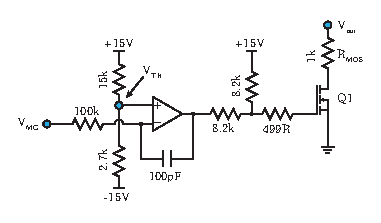
\includegraphics[width=\columnwidth]{fig/MOS.ai}
\caption{MOSFET ``quench'' circuit.
When the mid-ground node $\text{V}_\text{MG}$ (also shown in Fig.~\ref{Fig:PiezoCircuit}) goes below the threshold value set at $\text{V}_\text{TH}$, the op-amp puts the HV MOSFET Q1 into conduction.
When engaged, the time constant for capacitor $\text{C}_\text{out}$ in Fig.~\ref{Fig:PiezoCircuit} is given by $R_\text{MOS} C_\text{out}$, which for our circuit is set to \SI{1}{\milli\second}.
\label{Fig:MOS}}
\end{figure}

The high-voltage setpoint (absent voltages summed in at $\text{V}_\text{mod}$) is controlled by a low-noise DAC.
This has two advantages: digital control enhances setpoint repeatability, and makes it easy to integrate with a wide variety of computerized control electronics or implement more sophisticated servo loops.
While the modulation input $\text{V}_\text{mod}$ has a limited range of $\pm\SI{10}{\volt}$, larger voltage swings can be achieved by reprogramming the DAC.

As discussed in Section~\ref{Sec:NoiseAnalysis}, without modification the DAC would dominate the noise performance of $\text{V}_\text{out}$.
Therefore, we add a single-pole low-pass filter between $\text{V}_\text{ctl}$ and the non-inverting node of U2.
This filter has a switchable corner frequency (between \SI{165}{\hertz} and \SI{0.8}{\hertz}) to optimize noise performance at DC while still allowing for AC modulation when needed.

One downside of the flyback regulator presented above is that while the switched transformer is very efficient at charging the capacitor $\text{C}_\text{HV}$, discharge of the high-voltage line is limited by the $\approx\SI{1}{\second}$ RC time constant of the circuit.
To get around this limitation, we have added an auxiliary MOSFET ``quench'' circuit, as suggested in the DRV2700 datasheet, to quickly shunt $\text{V}_\text{out}$ to ground (see Figure~\ref{Fig:MOS}).
This circuit works by monitoring the voltage at $\text{V}_\text{MG}$, the mid-ground node controlled by op-amp U2.
If that voltage drops below a threshold set by $\text{V}_\text{TH}$, the comparator op-amp in Figure~\ref{Fig:MOS} changes the gate voltage of the MOSFET to put it into conduction.
The time constant for this configuration is given by $\tau \approx R_\text{MOS}\text{C}_\text{out}$. For our circuit, this changes $\tau$ to $\approx\SI{1}{\milli\second}$, allowing for the fast discharge of $\text{C}_\text{out}$. 
The threshold is $\text{V}_\text{TH} = \SI{-10.4}{\volt}$, but other values could be chosen depending on the design requirements.

\subsection{Auxiliary design features}
\label{Sec:AuxDesign}

Here, we discuss some additional features of our circuit that are independent of the high-voltage design but are advantageous for many applications.
The onboard microcontroller responsible for setting the DAC control voltage, $\text{V}_\text{ctl}$, also interfaces with frontpanel controls including a switch, LCD, and rotary encoder with an integrated push button.
The encoder/push button provide menu navigation, and the switch toggles between DC and scanning operation.
However, other user interfaces can easily be designed to work with the existing hardware.
Arduino-based code written in \CC defines the entire software interaction, and can be modified depending on the needs of the researcher.

The entire circuit fits into a standard Eurocard rack, which supplies power at $\pm\SI{15}{\volt}$.
While not required, the rack provides a backplane with analog lines to communicate with other modules (e.g., to implement a current feed-forward for laser diodes as described below).
We are presently designing a backplane with a secondary microcontroller that can be addressed over TCP/IP.
This vastly expands the conceivable control scenarios. 
For example, in our lab we implement a slow-feedback lock of two external-cavity diode lasers to a wavemeter.
LabView code on the computer attached to the wavemeter computes an error signal and corrective control voltage, which will be passed over our internal network to the piezo driver to correct for frequency drifts in the laser.
Other similar schemes are possible, enabling complete remote control of the laser electronics.

The modulation voltage $\text{V}_\text{mod}$ can be supplied either from a BNC on the frontpanel, or from the backplane.
This may be useful, e.g., with servo controllers that reside in the same rack as the other control electronics.
In either case, this voltage is differentially buffered to break ground loops.
An output voltage monitor (sensed at the inverting node of U2 in Figure~\ref{Fig:PiezoCircuit}, but not shown) is buffered and connected to a BNC on the frontpanel, an analog signal line on the backplane, and to the microcontroller\footnote{One drawback of this scheme is that the contribution of $\text{V}_\text{mod}$ is not sensed by the monitor. Future versions will instead monitor $\text{V}_\text{out}$ through a resistive divider, allowing the microcontroller to implement an infinite integrator and drive $\text{V}_\text{mod}$ to \SI{0}{\volt} in closed-loop operation. This will be a very useful feature to prevent the servo controller from railing.}.
%This enables the microcontroller to digitally implement an infinite integrator, driving $\text{V}_\text{mod}$ to \SI{0}{\volt} in closed-loop operation and preventing the servo controller from railing.
The backplane monitor could be fed to a low-noise current controller (e.g., one based on the design in~\cite{Erickson2008a}) to implement a laser diode current feed-forward.
The high voltage output is interlocked with another signal on the backplane, which can optionally be bypassed by placing an onboard jumper, permitting easy integration with existing laboratory interlock schemes if desired.
Further details on the design features discussed in this section, including sample software, can be found on Github~\cite{DesignFiles}.

\section{Noise Analysis}
\label{Sec:NoiseAnalysis}

\begin{figure}[t]
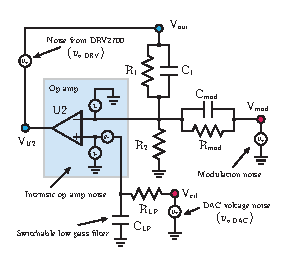
\includegraphics[width=\columnwidth]{fig/NoiseModel.ai}
\caption{Noise model (see text). The element labeled $Z_\text{LP}$ is comprised of a \SI{47}{\nano\farad} capacitor in parallel with a \SI{10}{\micro\farad} capacitor connected to ground through a switch, such that the corner frequency of the filter can be changed depending on the mode of operation. %The on-resistance of the switch introduces a zero in the transfer function at $\approx\SI{23}{\kilo\hertz}$, which has negligible effect on the computed RMS noise.
\label{Fig:NoiseModel}}
\end{figure}

\begin{figure}[t]
\subfloat{
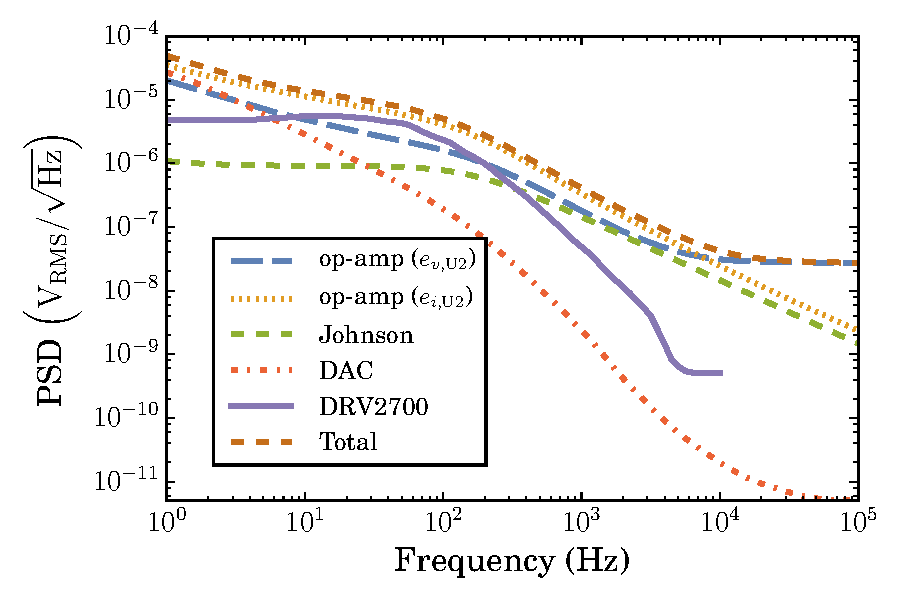
\includegraphics[width=\columnwidth]{fig/NoiseContrib.pdf}
}

\subfloat{
\centering
\begin{tabular*}{0.95\columnwidth}{@{\extracolsep{\fill}} lcc}
\hline\hline
\rule{0pt}{2.5ex}\multirow{2}{*}{Noise source} & RMS Voltage & RMS Voltage \\
& (\SI{1}{\hertz}~--~\SI{10}{\hertz})\rule[-1ex]{0pt}{1ex} & (\SI{10}{\hertz}~--~\SI{100}{\kilo\hertz})\rule[-1ex]{0pt}{1ex} \\
\hline
\rule{0pt}{2ex}$e_n$ (op-amp U2)  & \SI{26}{\micro\volt} & \SI{31}{\micro\volt}      \\
$i_n$ (op-amp U2)  &            \SI{51}{\micro\volt}     & \SI{73}{\micro\volt}      \\
DAC             &             \SI{28}{\micro\volt}    & \SI{8}{\micro\volt}       \\
Johnson-Nyquist &             \SI{3}{\micro\volt}    & \SI{31}{\micro\volt}        \\ 
\hline
\rule{0pt}{2ex}\textbf{total (calculated)} & \SI{64}{\micro\volt} & \SI{86}{\micro\volt}  \\
\hline\hline
\end{tabular*}
}
\caption{Noise Contributions (color online). Plotted are the noise contributions from each source in our model, along with the total calculated noise. Power spectral density (PSD) is referred to the high voltage output, and the table shows the integrated RMS noise due to each noise source in different frequency bands. The total RMS noise (summed in quadrature) over the entire \SI{1}{\hertz}~--~\SI{100}{\kilo\hertz} range is calculated to be \SI{107}{\micro\volt}. \label{Fig:NoisePlot}}
\end{figure}

We analyze the noise performance of the circuit according to the model shown in Fig.~\ref{Fig:NoiseModel}, where noise spectral densities are calculated at the node $\text{V}_\text{out}$.
A summary of each noise contribution (op-amp, DAC, Johnson-Nyquist, residual DRV2700) is shown in Fig.~\ref{Fig:NoisePlot}, along with the cumulative root-mean-square (RMS) nose estimates in different frequency bands.

To treat the intrinsic op-amp noise contributions, we first compute the noise gain $G_n$ for this amplifier configuration according to
\begin{align}
\label{Eq:NG}
G_n(s) &= 1 + Z_1\left(\frac{1}{R_2} + \frac{1}{Z_\text{mod}}\right)\,,
\end{align}
with equivalent impedances $Z_1 = R_1/(1+R_1 C_1 s)$ and $Z_{\text{mod}} = R_{\text{mod}}/(1+R_{\text{mod}} C_{\text{mod}} s)$, and where $s$ is the Laplace variable.
By design, we've chosen $Z_1 \equiv Z_{\text{mod}}$ such that the signal gain from the node $\text{V}_{\text{mod}}$ is unity.
This reduces Eq.~(\ref{Eq:NG}) to
\begin{align}
\label{Eq:RedNG}
G_n(s) &= 2 + \frac{Z_1}{R_2}\,.
\end{align}

The op-amp noise is parametrized by two noise contributions: $e_n$, the input voltage noise power spectral density (PSD), and $i_n$, the input current noise PSD.
For the LM7171, $e_n = \SI[per-mode=symbol]{14}{\nano\volt\per\sqrthz}$ and $i_n = \SI[per-mode=symbol]{1.5}{\pico\ampere\per\sqrthz}$ at $\SI{10}{\kilo\hertz}$, with a $1/f$ noise character below this frequency~\cite{LM7171Datasheet}.
The voltage noise is summed in at the non-inverting input, while the current noise is present at both inputs.
To convert $i_n$ to an equivalent voltage noise $e_n$, we multiply by the impedances $Z_n$ and $Z_p$ seen by the inverting and non-inverting nodes, respectively.
These are calculated as
\begin{align}
\begin{split}
\label{Eq:ZnZp}
Z_n &\equiv \left(\frac{1}{Z_1} + \frac{1}{Z_\text{mod}} +  \frac{1}{R_2}\right)^{-1}   = \frac{Z_1 R_2}{2R_2 + Z_1} \\
Z_p &\equiv \left(\frac{1}{R_\text{LP}} + \frac{1}{Z_\text{LP}}\right)^{-1}\,.
\end{split}
\end{align}
The impedance $Z_\text{LP}$ is determined by the corner frequency of a switchable low-pass filter between the DAC and the non-inverting node of U2 (discussed below).
The total noise contribution of the op-amp U2 (referenced to the output) is
\begin{align}
\label{Eq:OpAmpNoise}
e_{n,\text{U2}} &= G_n(s)\sqrt{e_n^2 + (Z_n i_n)^2 + (Z_p i_n)^2}\,.
\end{align}

Next, we calculate the noise contribution from the DAC.
The noise signal gain from the node $\text{V}_{\text{ctl}}$ is given by
\begin{align}
\label{Eq:Gdc}
G_{\text{ctl}} &= \left(\frac{Z_\text{LP}}{R_\text{LP} + Z_\text{LP}}\right)G_n(s)\,,
\end{align}
where the first term represents the contribution to the transfer function from the switchable low-pass filter.
Without the addition of this low-pass filter, the voltage noise of the DAC would dominate both the low- and high-frequency noise performance of the circuit.
A simple solution would be to place a fixed-corner filter at this node, but this would severely restrict the AC performance of $\text{V}_\text{ctl}$.
Thus, we use a switchable low-pass filter (as described in Sec.~\ref{Sec:SlowModulationMOS}) to achieve low-noise performance during DC operation, while still permitting the DAC to modulate $\text{V}_\text{ctl}$ more quickly when needed.
In our circuit, the high-corner filter is comprised of a \SI{20.5}{\kilo\ohm} resistor and \SI{47}{\nano\farad} capacitor, with $f_c \approx \SI{165}{\hertz}$.
In DC mode, a secondary \SI{10}{\micro\farad} capacitor in parallel with the \SI{47}{\nano\farad} capacitor mentioned above can be connected to ground through a low resistance digital switch.
This changes the corner frequency to \SI{0.8}{\hertz}.
The non-zero resistance of the switch contributes a zero to the transfer function at $\approx\SI{23}{\kilo\hertz}$, but has negligible effect on the performance.
The DAC voltage noise contribution can now be calculated as $e_{n,\text{DAC}} = G_{\text{ctl}} v_{n,\text{DAC}}$, where $v_{n,\text{DAC}}$ is the frequency dependent output voltage noise of the DAC. 
In subsequent calculations, we take the DC mode operation for the switchable low-pass filter.
%The DAC used in our design (Analog devices, AD5663R) has a white noise floor of \SI[per-mode=symbol]{100}{\nano\volt\per\sqrthz} with an $\approx\SI{1}{\kilo\hertz}$ corner frequency.

The low-noise stabilization circuit is limited in its ability to reject residual switching noise from the DRV2700 regulator and passive filtering by the total loop gain analyzed from node $\text{V}_\text{out}$.
The LM7171 has an open-loop gain of \SI{85}{\decibel} ($\approx 1.8\times 10^4$), with a dominant pole at $\approx\SI{10}{\kilo\hertz}$\cite{LM7171Datasheet}.
We model the open loop gain, $G_\text{OL}$, as
\begin{align}
G_\text{OL} &= \frac{1.8\times10^4}{1+s/(2\pi\cdot\SI{10}{\kilo\hertz})}\,.
\end{align}
The contribution of this residual switching noise, $v_{n,\text{DRV}}$, to the output is given by
\begin{align}
e_{n,\text{DRV}} &= \frac{v_{n,\text{DRV}}}{1+G_\text{OL}\left(\frac{R_2||Z_\text{mod}}{Z_1 + R_2||Z_\text{mod}}\right)}\,.
\end{align}
For $R_1=\SI{1}{\mega\ohm}$ and $\text{C}_1 = \SI{1}{\nano\farad}$, $v_{n,\text{DRV}}$ is attenuated by as much as \SI{76}{\decibel} at \SI{6.3}{\kilo\hertz}, with a rolloff of \SI[per-mode=symbol]{10}{\decibel\per\text{decade}} at higher frequencies.
(INCLUDE DRV NOISE MODEL IN CALCULATION?? -- EG, WHAT ORDER DO THEY CONTRIBUTE?)

% such that the closed-loop gain for noise contributed by the flyback regulator at node $\text{V}_\text{out}$ is minimized in the \SIrange{40}{100}{\kilo\hertz} switching noise band.
%For $R_1=\SI{1}{\mega\ohm}$, we choose $\text{C}_1=\SI{1}{\nano\farad}$.
%The noise gain 

Given the noise model discussed above, our circuit is dominated by Johnson noise at intermediate to high frequencies, and the op-amp's intrinsic current noise at lower frequencies.
Both of these contributions could be suppressed by using lower resistances $R_1$ and $R_\text{mod}$, however one must be careful about power and current limitations when dealing with such high voltages.
Each noise source is tabulated and plotted in Fig.~\ref{Fig:NoisePlot}, and the total voltage noise  is calculated to be $\SI{107}{\micro\volt}$ ($\SI{1}{\hertz} - \SI{100}{\kilo\hertz}$).
Frequency-dependent input noise parameters in this model were extracted from datasheet spectral density curves\cite{SHEETS}.

\section{Results}
\label{Sec:Results}
\begin{figure}[t]
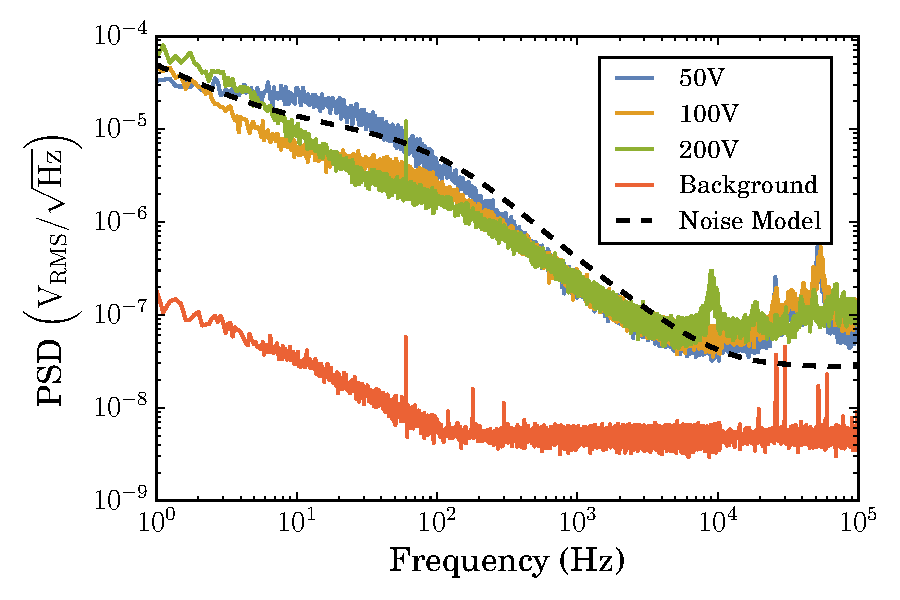
\includegraphics[width=\columnwidth]{fig/VoltagePSD.pdf}
\caption{Voltage power spectral density at various output voltages. The integrated RMS voltage noise ($\SI{1}{\hertz} - \SI{100}{\kilo\hertz}$) is $\{138, 80, 101\}~\si{\micro\volt}$ measured at  $\{50, 100, 200\}~\si{\volt}$, with no output load. \label{Fig:PSD}}
\end{figure}

The measured performance of the high-voltage piezo driver is shown in Fig.~\ref{Fig:PSD}, where we plot the noise power spectral density measured at several different output voltages.
These traces were taken on a Stanford Research Systems SR780 spectrum analyzer, with the high-voltage output coupled through a \SI{0.5}{\hertz} high-pass filter and without any capacitive load.
This represents a worst-case scenario, as larger capacitances at the output will reduce the noise.
The integrated noise ($\SI{1}{\hertz} - \SI{100}{\kilo\hertz}$) was measured to be $\{\SI{138}{\micro\volt}_\text{RMS},~\SI{80}{\micro\volt}_\text{RMS},~\SI{101}{\micro\volt}_\text{RMS}\}$ for \{\SI{50}{\volt}, \SI{100}{\volt}, \SI{200}{\volt}\} outputs. 
This matches well with the expected total RMS noise calculated in Section~\ref{Sec:NoiseAnalysis}.
DISCUSS WHY 50V IS WORSE

Figure~\ref{Fig:TimeDomain} shows the performance at both short- and long-time scales.
At long times, voltage fluctuations on the order of a few \si{\milli\volt} can be observed.
This is due generically to $1/f$ noise, but also correlates with the external temperature.
A cross-correlation between measured temperature and output voltage (trace not shown) yields an effective temperature coefficient of \SI[per-mode=symbol]{-24}{ppm\per\celsius} at \SI{100}{\volt}.
The short-term trace was taken on a PicoScope~5442B (ac-coupled, \SI{100}{\volt} output).
Points are colored based on their normally distributed statistical probability, and thus give a visual estimation of the RMS width.

\begin{figure}[t]
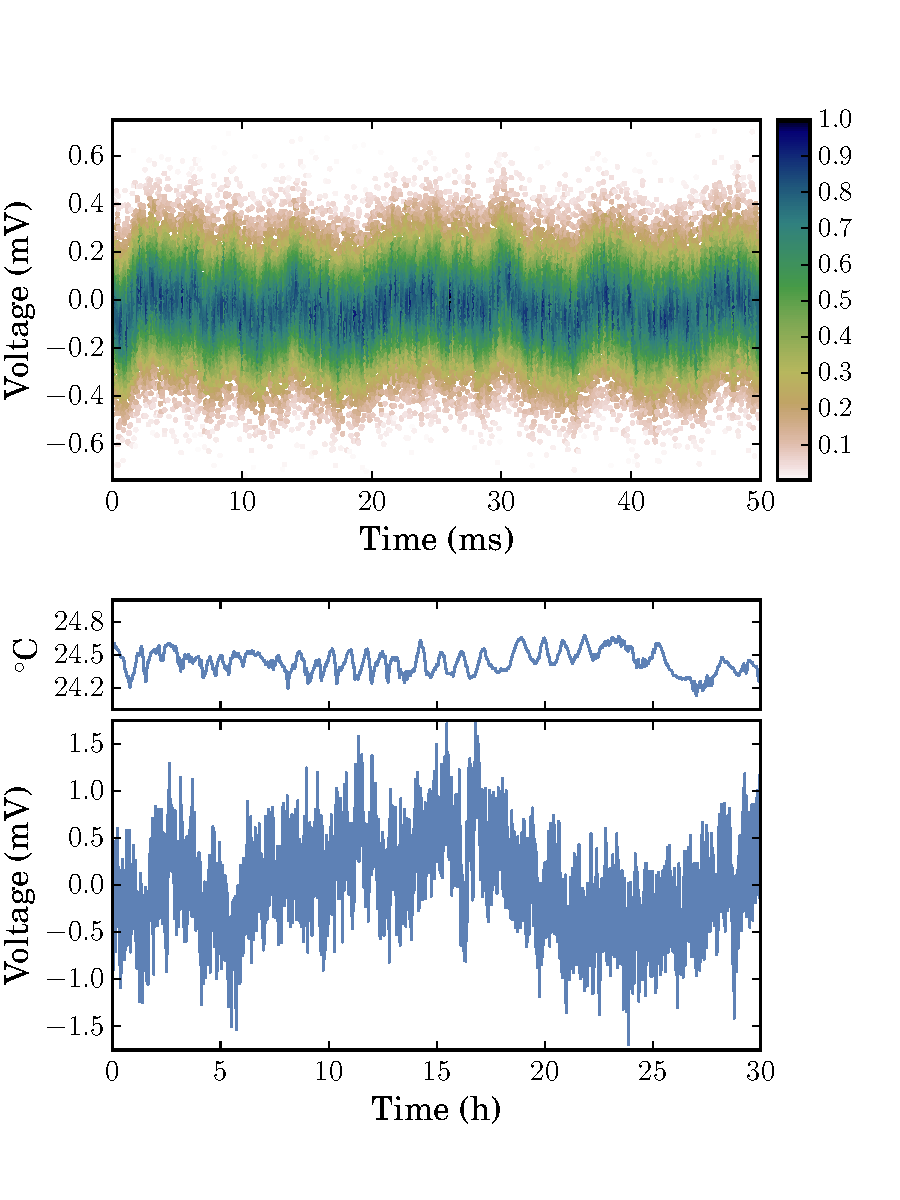
\includegraphics[width=\columnwidth]{fig/TimeDomain.pdf}
\caption{Time-domain traces of the high voltage output (\SI{100}{\volt}). (a) Short-time scatterplot  (AC coupled). Points are colored based on the Gaussian spread in acquired voltages, thus indicating the RMS width of the trace. (b) Long-term trace, measured on a Keithly~2010 digital multimeter. A~\SI{100}{\volt} DC offset is subtracted from the plotted values. The top panel shows the lab temperature during the same time period.\label{Fig:TimeDomain}}
\end{figure}

Figure~\ref{Fig:TransferFunc} shows the measured frequency response under different load conditions. The unloaded bandwidth is as high as a few megahertz, while a \SI{1}{\micro\farad} capacitive load can still be driven at $\approx\SI{100}{\kilo\hertz}$. 
Several mechanical resonances can be seen with a \SI{700}{\nano\farad} piezoelectric load, as expected.
In a laboratory setting, these resonances can be mitigated by using a digital feedback controller with notch filters tuned to match the exact resonance frequencies observed in the system\cite{Ryou2016a}, thereby extending the usable bandwidth out to $\approx\SI{100}{\kilo\hertz}$.
\begin{figure}[t]
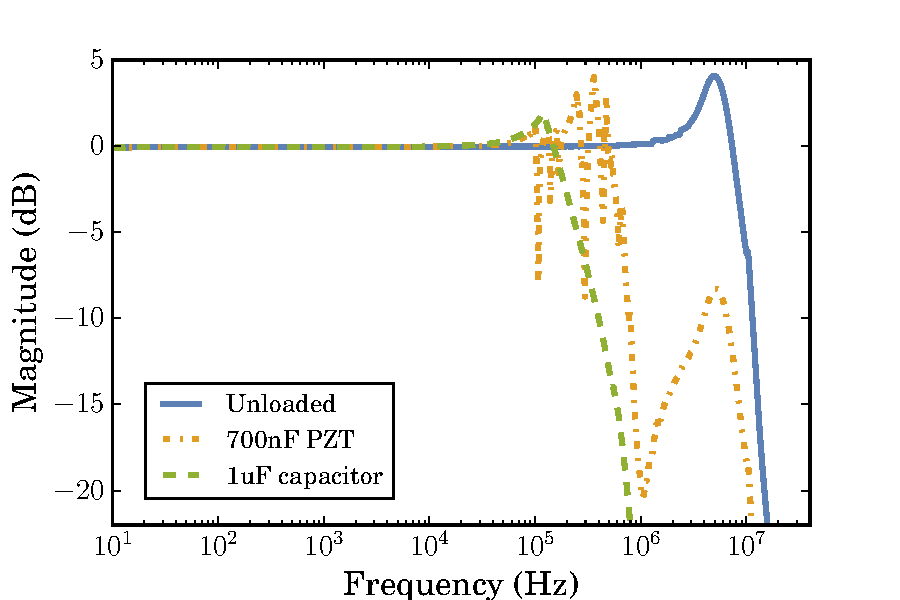
\includegraphics[width=\columnwidth]{fig/PiezoModulationTransfer.pdf}
\caption{Modulation input transfer function (color online). The blue line indicates the unloaded frequency response, while the dash-dotted orange trace shows the response with a ThorLabs piezoelectric actuator {(PN~AE0505D08F)}. Mechanical resonances above $\approx\SI{50}{\kilo\hertz}$ are clearly visible. The dashed green trace shows the response under a \SI{1}{\micro\farad} purely capacitive load. Loaded response bandwidth is $\approx\SI{100}{\kilo\hertz}$, while the unloaded bandwidth is $\approx\SI{1}{\mega\hertz}$.\label{Fig:TransferFunc}}
\end{figure}

\section{Conclusion}
\label{Sec:Conclusion}

We have designed, built, and characterized a high-voltage piezoelectric driver optimized for use in a modern atomic physics laboratory.
It is based on a flyback configuration switching regulator, but is able to achieve very low noise performance by active stabilization from a high slew-rate op-amp.
This hybrid architecture makes it small and easy to deploy in a variety of situations, without requiring an external, bulky high-voltage power supply.
The design principles discussed here can be adapted to fit the exact application, and all design files are freely available on GitHub for others to use and modify.

The authors would like to thank Z. Smith for useful discussions.
This work was partially supported by the Office of Naval Research, and the National Science Foundation through the Physics Frontier Center at the Joint Quantum Institute.

%
%\section{Other...}
%\begin{itemize}
%\item $1/f \rightarrow$ white noise corner frequency
%\item white noise spectral density
%\item RMS noise (0.1 - 10 Hz; 10 Hz - 10 kHz, or something similar) -- use SRS voltage preamp?
%\item How effective is the LM7171 at reducing switching noise? look at FFT power before final filter resistor, and at output of op amp (dBc spec)
%\item compare noise to predicted values
%\item longterm trace on kiethly -- across voltage divider at output? Monitor vs temperature? -- need to find low Tc resistors, at least.
%\item see what dependence is on power source -- eg, JQI power supply vs lab supply vs very quiet voltage regulator?
%\item current draw -- display in some ``bottom line'' specs table?
%\item bandwidth measurements -- full scale triangle ramp, small signal bandwidth -- discuss limitations on this (eg, also versus different piezo loads)
%\item Lock a laser, show RMS noise fluct vs. old piezo?
%\item compare to SC100 toptica controller? even if just internally.
%\end{itemize}


% If in two-column mode, this environment will change to single-column format so that long equations can be displayed.
% Use only when necessary.
%\begin{widetext}
%$$\mbox{put long equation here}$$
%\end{widetext}

% Figures should be put into the text as floats.
% Use the graphics or graphicx packages (distributed with LaTeX2e). EPSFig is no longer fully supported.
% See the LaTeX Graphics Companion by Michel Goosens, Sebastian Rahtz, and Frank Mittelbach for examples.
%
% Here is an example of the general form of a figure:
% Fill in the caption in the braces of the \caption{} command.
% Put the label that you will use with \ref{} command in the braces of the \label{} command.
%
% \begin{figure}
% \includegraphics{}% % Important NOTE: Please make certain your figures do not include local directory paths. ex. "c:\file\sub\fig1.eps"
% \caption{\label{}}%
% \end{figure}

% Tables may be be put in the text as floats.
% Here is an example of the general form of a table:
% Fill in the caption in the braces of the \caption{} command. Put the label
% that you will use with \ref{} command in the braces of the \label{} command.
% Insert the column specifiers (l, r, c, d, etc.) in the empty braces of the
% \begin{tabular}{} command.
%
% \begin{table}
% \caption{\label{} }
% \begin{tabular}{}
% \end{tabular}
% \end{table}

% If you have acknowledgments, this puts in the proper section head.
%\begin{acknowledgments}
% Put your acknowledgments here.
%\end{acknowledgments}

% Create the reference section using BibTeX:
%\bibliographystyle{jabbrv_abbr}
\bibliography{references}
% Run this once to generate your BBL file. Then copy the contents of your BBL file into your main latex file, commenting out "\bibliography"

\end{document}
%
% ****** End of file aiptemplate.tex ******
